Information relevant for decision making in agriculture can be extracted from heterogeneous remote sensing, environmental and intervention-derived data by means of machine learning. With advancements in computational technologies, the development and training of non-linear multilayer algorithms has become feasible. These methods are commonly referred to as deep learning. Probably the most widely used deep learning structure is that of CNNs, proved to be superior in a variety of image analysis tasks. Other common structure is the RNN network, which is used for modelling sequences of data. A common property of the deep learning structures is that training of the models is performed based on data, i.e., no predefined and pre-calculated feature vector is needed. This, however, implies that extensive data sets are required for training the models and the operation principles of the models are usually not revealed. Figure~\ref{fig:ii-AgroAI_Topics} depicts some application areas of deep learning in agriculture.

\begin{figure}[htb]
    \centering
    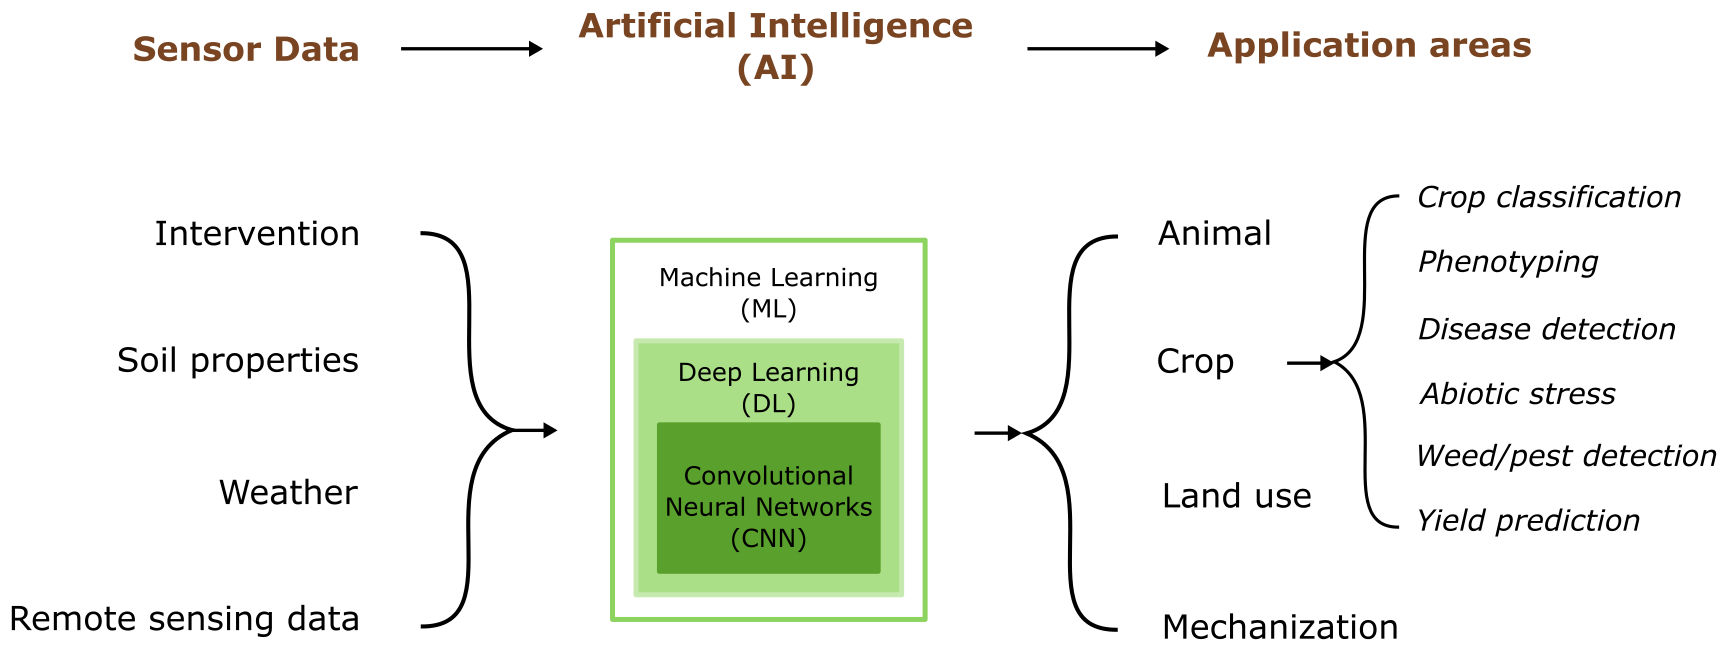
\includegraphics[width = 0.8\textwidth]{images/ii-AgroAI_Topics.png}
    \caption{Application areas of DL in agriculture.}
    \label{fig:ii-AgroAI_Topics}
\end{figure}

Remote sensing data can be acquired from satellites such as ESA’s Sentinel-2, for example. The problem with the satellite data is that if there is a cloud cover during the overflight of the satellite, no useful data are obtained. The spatial resolution of Sentinel-2 imagery is at best 10 m, which is enough for many applications but too low to allow using texture-based information in the images. Using UAVs for data acquisition offers better spatial resolution, the data acquisition time can be selected by the user and the data can be acquired also in cloudy conditions. Spectral wavelengths can be selected by using appropriate camera; UAV-mountable RGB-NIR cameras are available at affordable price. The drawback is that the UAV has to be operated locally and managing the data and extracting relevant information requires highly specialized skills.


\section{Deep learning and intra-field yield prediction}

The studies described in the publications [I], [II] and [IV] seek to predict yield at the intra-field scale using UAV based images in order to estimate yield variance within the field. This is in contrast to studies utilizing satellite-based, medium to low resolution data and predicting for considerably larger areas at lower spatial resolution. Models at intra-field scale offer the individual farmer the possibility of in-season monitoring of crop, which enables decision support systems for interventions necessary to achieve higher yields. 

Publication [I] is an important first step towards establishing a combined model for wheat and barley yield prediction in the Finnish continental subarctic climate. The long summer growing days in this region present a unique profile of temperature and photoperiod, justifying a region-specific deep learning model for these crops. By collecting high-resolution, namely 0.31 $\times$ 0.31 m/px, data using commercial off-the-shelf UAV and camera packages, the attention was focused on a spatial scale that enables us to predict intra-field yield variation within the context of individual farm crop monitoring. Considering that [I] models the yield based only on images, the resulting prediction error of 484 kg/ha test MAE, 8.8 \% test MAPE and 0.857 $R^2$-score is promising. The results of [I] indicate that the CNN models are capable of reasonable accurate yield estimates based on RGB images. This suggests that multiple spectral bands increase the information content in comparison to the condensed NDVI raster. From the results of [V] it can be suggested that complementing the RGB data with NIR channel might further enhance the prediction capabilities of the CNN model. Additionally, NIR-based vegetation indices could have improved modelling performance even more as discussed in \cite{Zhao2020}. Intra-field crop yield prediction based on multispectral UAV data based is, thus, a subject for a future study.

As further examined in [II], the case study with the CNN from [I] revealed some limitations of the model in yield prediction. The model underestimated/overestimated the yield in the regions of high/low yield values, respectively. Another limitation is related to yield data pre-processing. In some cases the polygons of yield data overlap causing errors in yield density maps.
 
In [IV] the feasibility of using spatiotemporal deep learning architectures in modelling crop yield at the intra-field scale was evaluated using high-resolution UAV data. With full sequence modelling, a 3D-CNN based architecture performed the best with 218.9 kg/ha test MAE, 5.51\% test MAPE and 0.962 test R$^2$-score. Compared to [I] using just a point-in-time single frame predictor with 484.3 kg/ha MAE and 8.8\% MAPE, the modelling performance was improved by 265.4 kg/ha MAE (54.8\% improvement) and 3.29\% MAPE (37.4\% improvement) with time series inputs. With a shorter sequence the 3D-CNN model attained 292.8 kg/ha test MAE, 7.17\% test MAPE and 0.929 test R$^2$-score. As weather information was utilized in [IV] at city scale, the accuracy of the growth phase could be further improved with specifically located weather stations. Weather stations located in the approximate vicinity of the fields under scrutiny could provide better and more accurate measurements of the local temperatures and other climatological variables and thus might help the model produce even better predictions when sequences are involved. This was corrected in [V] by using two distinct weather stations located near the studied fields.

These results with point-in-time and multitemporal models are competitive in light of recent yield prediction studies. Sun et al. \cite{Sun2020} utilized UAVs to gather hyperspectral data of potato tuber growth at the resolution of 2.5 cm/px. They utilized traditional ML methods, such as linear models and decision trees, to perform tuber yield estimation using individual data points gathered in-season at the intra-field scale, achieving 0.63 R$^2$-score for the tuber yield prediction accuracy with a Ridge regression. Lee at al. \cite{Lee2020} used an UAV to collect multispectral data from wheat and corn fields to estimate intra-field crop nitrogen content using linear regression and point samples - spatial features were not utilized. They fit multiple linear models to wheat and corn and attained 0.872 R$^2$-score on average. Fu et al. \cite{Fu2020} performed wheat leaf area index and grain yield estimation with various vegetation indices derived from point-in-time multispectral UAV data using multiple machine learning methods, neural networks included. The highest performance they attained was 0.78 R$^2$-score with a random forest model. However, they fed the input data as point samples. Performing county-scale soybean yield prediction, \cite{Sun2019} used a CNN, an LSTM and a composite CNN-LSTM to model soybean yield with in-season satellite data. They achieved an average 0.78 R$^2$-score with the spatiotemporal CNN-LSTM model. \cite{Yang2019} utilized RGB and multispectral data acquired with a UAV from rice fields in China to predict rice yields with a composite CNN model on field block scale. Feeding the multisource data to distinct, parallelized CNNs, they report a rice yield prediction performance of 0.50 R$^2$ and 26.6\% MAPE.

In their study, Sun et al. \cite{Sun2020} used input data with resolutions from 500 $\times$ 500 m/px to 1 $\times$ 1 km/px. Rustowicz et al. \cite{Rustowicz2019} performed crop type classification in Europe and Africa with multi-temporal satellit data at resolutions from 3 $\times$ 3 m/px to 10 $\times$ 10 m/px. They attained F1 scores 91.4 for the CNN-ConvLSTM and 90.0 for the 3D-CNN, averaged over crop types in their Germany data set. Yaramasu et al. \cite{Yaramasu2020} performed pre-season crop type mapping for the area of Nebraska, US, employing a CNN-ConvLSTM to extract spatiotemporal features from multi-temporal multi-satellite composite data set. Using prior years of crop type related data to predict a map of crop types, they attained an average accuracy of 77\% across all crop types in their data. The data was processed to a resolution of 30 $\times$ 30 m/px. Ji et al. \cite{Ji2018} utilized a 3D-CNN to classify crop types from multi-temporal satellite data gathered from an area within China, acquiring a classification accuracy of 98.9\% with the model. Their input data resolutions were from 4 $\times$ 4 m/px to 15 $\times$ 15 m/px. Borra-Serrano et al. \cite{Borra-Serrano2020} performed weekly UAV image collections in a controlled field experiment with soybeans, performing seed yield prediction with multiple linear models fit to the multi-temporal data. Thus, spatiotemporal modelling with novel techniques was not performed. With seed yield prediction, they achieved 0.501 adjusted R$^2$ score. The resolution of their data was 1.25 $\times$ 1.25 cm/px.

In [I] and [II] it is shown that with high-resolution UAV data, crop yield prediction with CNNs is feasible and produces results accurate enough for performing corrective farming actions in-season. In [IV] it is shown that adding time as an additional feature not only improves the modelling performance with high-resolution UAV RGB data but also improves the predictive capabilities. Additionally, using weekly UAV data gathered during the first month provides enough data for the model to build an accurately predicted yield map from which to draw further conclusions. The use of both high-resolution point-in-time and multitemporal remote sensing data is beneficial in crop yield modelling and prediction with deep learning. Furthermore, the easy accessibility of commercially available UAVs with mounted RGB sensors enables image data acquisition in higher resolutions compared to satellites. This in turn opens up the possibilities to perform modelling and predictions at intra-field scale. As shown in the publications [I], [II] and [IV], the use of UAV-based data and proper spatiotemporal deep learning techniques is an enabler of more sophisticated decision support systems in the domain of agriculture. 

\section{Multisource input data assessment}

In [V], the effects of using input data from multiple sources on the task of spatial crop yield prediction were evaluated. The performance with larger number of fields using UAV RGB data had already been extensively studied in [I] and [IV]. Thus, training a model with only UAV RGB data provides a studied baseline to which models trained with additional data can be compared against. The best performing data configuration was \emph{S2 Full} with 364.1 kg/ha test RMSE, 5.18\% test MAPE and 0.922 test R$^2$ using all 39 layers of input data for each extracted frame (see Section 3 of publication [V]). Compared to the baseline \emph{RGB Only} model, the \emph{S2 Full} attained 65.6\% lower RMSE, 67.3\% lower MAE, 71.5\% better MAPE and 0.579 higher R$^2$ with the test set. Generally every model with multisource inputs performed better than the baseline model.The study indicates that increasing the number of input data sources increases the performance of intra-field crop yield prediction. To draw definite conclusions on the most optimal configuration of input data sources more data is required. With more representative data, generalizable conclusions are more warranted. The relative improvement compared to baseline of using UAV RGB only as the input data were notable. Consolidating UAV RGB data with soil information and ground topology data already somewhat improves the prediction performance, while largest performance gains were gained from using Sentinel-S2 in addition to UAV RGB, soil sampling, Veris MSP3 soil scanner, weather and topography data. As the data in [V] focuses on a single growing season, the generalization of a multisource crop yield prediction model with multiple years of data is a subject for a future study.

The study of publication [III] indicates that the random forest model outperforms the Sentinel-2 CLDPRB and SCL data layers in detecting cloudy areas ($y = 0$). For non-cloudy areas the detection accuracy was slightly higher for the Sentinel products. The developed method was found to improve the usability of Sentinel data in crop monitoring. By visual inspection it was observed that in many cases when the Sentinel-2 products indicated the whole crop field to be cloud-covered, there were still significant areas of almost clear skies. The proposed algorithm proved capable in detecting these areas with considerable accuracy. The classification results are further usable in different applications. Firstly, commercial applications routinely utilize satellite data based NDVI maps, which greatly benefit from accurate estimations of pixel-wise cloud canopy. Another application is in preprocessing satellite data used as inputs for crop yield estimation.


\section{Limitations}

A limitation to our crop yield estimation studies is the use of aggregated crop type data collected from various fields. Using a single model to predict for wheat, barley and oats prohibits both the inference and the performance analysis of the model on a per-crop basis. Additionally, the remote sensing data based modelling approach doesn't take into account any existing crop growth models. Those could well be utilized to further provide better performance, akin to what has been done in \cite{Borra-Serrano2020}.

Models trained at large regional scales rarely extrapolate to finer scales, though efforts have been taken to develop scalable models \cite{Donohue2018}. A good strategy of dividing the data into training, validation and testing sets on field basis would be required to prove that models are capable to generalize. This raises an important discussion point regarding how the frames were extracted in publications [I], [II], [IV] and [V], especially considering the overlap of data across adjacent frames. The frames were randomly allocated to training and test sets. Another important point related to input sample independence is the invariability of data from distinct sources. This is issue is specific to [V], where input samples contain both temporally and spatially invariable data. Temporally invariable data includes soil samplings, Veris MSP3 soil scanner data and topographical maps. Weather data, on the other hand, is spatially constant. While the cumulative temperatures and rain sums do change in time, the time-specific weather layers are effectively rasters with constant values. Whether the input data is split spatially or temporally to training and test sets, there is a case to be made that some data might be present in similar form in all split data sets simultaneously. With traditional machine learning, such as linear models, data which is not independent and identically distributed would require extensive prior work to find feature-wise couplings. As pointed out in \cite{Sun2019}, neural networks learn these couplings implicitly from the data. Thus, the input layers are not handled in solitude one by one but are always utilized in the context of other data present in an input sample. The context includes spatial, temporal and inter-channel dimensions. Therefore, the test data as a combination of inputs can be considered distinct from training and validation sets. This is further reinforced by the results of [V]. The performance gains with UAV RGB data combined with temporally invariant soil information and ground data is trumped by the performance gains of data configurations using Sentinel-S2 data as additional inputs. This would suggest that the combination of the inputs matters more than presence of distinct, invariant data in training, validation and test sets. 

Regarding multisource data in the context of smart farming and crop yield estimation, data itself is an evolving research topic. The use of multisource inputs in remote sensing, while focusing on multispectral data acquired from satellite systems orbiting the globe, has been extensively reviewed in \cite{Ghamisi2019}. The use of multispectral data from UAVs and the prediction architectures thereof is also a developing topic \cite{Messina2020}. Another topic related to spatial data is that of autocorrelation \cite{Amgalan2020}. To address autocorrelation of spatial frames in a future study, the inclusion of pixel-wise location information, as suggested in \cite{Amgalan2020}, should be sufficient to inform the deep learning model whether data similarity is due to proximity or some other factor or combination of them.

Several issues should be considered with cloud cover classification in [III]. Firstly, when training the random forest classifier, the thresholded absolute difference between the Sentinel-2 and drone data was used as the ground truth. While it can be argued that the main cause of this difference is cloudiness, there may also be other factors involved such as shadows or differences in irradiance. The satellite and drone imagery were not necessarily acquired during the same time of the day or same day of the week, although best time-matching pairs were looked for when selecting the data. In some cases a couple of days may cause significant changes in the crop development. Another limitation comes from using the NDVI data layers for ground truth assessment. While the NDVI index contains significant information for vegetation monitoring and is probably a good choice when assessing cloud cover in crop fields, its use reduces the generalizability of the results to other land cover types. 

\section{Conclusions}

In summary, it is shown in [I] and [II] that with high-resolution UAV data, crop yield prediction with CNNs is feasible and produces results accurate enough for performing corrective farming actions in-season. In [IV] it is shown that adding time as an additional feature (time series data) not only improves the modelling performance (post-season prediction) with high-resolution UAV RGB data but also improves the predictive capabilities (in-season prediction). Additionally, using weekly UAV data gathered during the first month provides enough data for the model to build an accurately predicted yield map from which to draw further conclusions. The use of both high-resolution point-in-time and multitemporal remote sensing data is beneficial in crop yield modelling and prediction with deep learning. Furthermore, the easy accessibility of commercially available UAVs with mounted RGB sensors enables image data acquisition in higher resolutions compared to satellites. This in turn opens up the possibilities to perform modelling and predictions at intra-field scale. As shown in the publications [I], [II] and [IV], the use of UAV-based data and proper spatiotemporal deep learning techniques is an enabler of more sophisticated decision support systems in the domain of agriculture. Furthermore, the study presented in [V] shows that using various data sources for crop yield prediction in addition to UAV RGB data improves the predictive capabilities of the model. Referring to the use of specialized equipment in data acquisition, limiting the data sources to those common to majority of fields would, however, ensure better generalization capabilities for the models. Finally, as shown in [III], data based modelling can also be employed to perform quality assurance for satellite based data used in yield estimation and other relevant application contexts. 